% !TEX root = relative/or/absolute/path/to/root/file.tex
% Document class and font size
\documentclass[a4paper,10pt]{extarticle}

% Packages
\usepackage[utf8]{inputenc} % For input encoding
\usepackage{geometry} % For page margins
\geometry{a4paper, margin=0.75in} % Set paper size and margins
\usepackage{titlesec} % For section title formatting
\usepackage{enumitem} % For itemized list formatting
\usepackage{hyperref} % For hyperlinks
\usepackage{kotex}
\usepackage{graphicx}
\usepackage{array}
\usepackage{longtable}
\usepackage{float}
\usepackage{lipsum}
\usepackage{multicol,tasks}
\usepackage[skip=3pt]{caption}

% Formatting
\setlist{noitemsep} % Removes item separation
\titleformat{\section}{\large\bfseries}{\thesection}{1em}{}[\titlerule] % Section title format
\titlespacing*{\section}{0pt}{\baselineskip}{\baselineskip} % Section title spacing
\graphicspath{{../../pictures}}

% Begin document
\begin{document}
% Disable page numbers
\pagestyle{empty}
% Enable page numbers
% \pagenumbering{arabic}

% Header

% \begin{minipage}{\textwidth}

\begin{minipage}{0.1\textwidth}
	\begin{flushleft}
		\includegraphics[height=4.5cm]{photo_dlicense.jpeg}
	\end{flushleft}
\end{minipage}
\hfill
\begin{minipage}{0.7\textwidth}
	\begin{flushright}
		\textbf{\Large 이현빈, Hyeonbeen Lee} % Name
		\newline\newline
		\begin{tabular}{rl}
			\textbf{Mobile: }         & \href{tel:+82-10-6236-4693}{+82-10-6236-4693}                                                                 \\
			\textbf{Instagram: }      & \href{https://www.instagram.com/leehyeonbeen}{@leehyeonbeen}                                                  \\
			\textbf{EMail: }          & \href{mailto:edward.hyeonbeen.lee@gmail.com}{edward.hyeonbeen.lee@gmail.com}                                  \\
			\textbf{GitHub: }         & \href{https://github.com/leehyeonbeen}{github.com/leehyeonbeen}                                               \\
			\textbf{Google Scholar: } & \href{https://scholar.google.com/citations?user=TiduRxoAAAAJ}{scholar.google.com/citations?user=TiduRxoAAAAJ} \\
			\textbf{LinkedIn: }       & \href{https://www.linkedin.com/in/hyeonbeen-lee-239500286/}{linkedin.com/in/hyeonbeen-lee-239500286}
		\end{tabular}
		% \end{center}
	\end{flushright}

\end{minipage}
% \end{minipage}


% Education Section
\newcolumntype{L}{>{\raggedright\arraybackslash}m{1.6cm}}
\newcolumntype{R}{>{\centering\arraybackslash\small}m{3cm}}
\renewcommand*{\arraystretch}{1.5}
\noindent
\section*{인적사항}
\begin{center}
	\vspace*{-0.8cm}
	\noindent
	\begin{longtable}{LRLRLR}
		\textbf{성명:}   & 이현빈                   & \textbf{생년월일:} & 1996.07.04 (양력) & \textbf{병역사항:}  & 해병병장 만기전역 \small{(2017.05$\sim$2019.02)} \\
		\hline
		\textbf{주소:}   & 서울특별시 용산구 회나무로39길 6-3 & \textbf{구사언어:} & 한국어, 영어, 일본어    & \textbf{신체사항: } & 189cm / 62kg                             \\
		\hline
		\textbf{지원분야:} & {샵 아모멘토 운영팀 바잉 어시스턴트}
	\end{longtable}
\end{center}


% \textbf{성명}, 과학중점과정 \hfill 입학: 2012.03 | 졸업: 2015.02
% \newline
% \textbf{경희대학교}, 기계공학과 \hfill 입학: 2015.03 | 졸업: 2022.02\\ % University name and location
% 학사학위 (학위지도교수: 정신규, 김진균)\hfill 전체학점: 3.87/4.5 | 전공학점: 3.84/4.5\\ % Degree and GPA
% 학위논문명: \textit{\small{Data-driven aerodynamic coefficient prediction using}}\\
% \hspace*{1.9cm}\textit{\small{deep neural
%         network and PARSEC airfoil parameterization}}

% Education Section
\section*{학력사항}
\noindent
\textbf{반포고등학교}, 과학중점과정 \hfill 입학: 2012.03 | 졸업: 2015.02
\newline
\textbf{경희대학교}, 기계공학과 \hfill 입학: 2015.03 | 졸업: 2022.02\\ % University name and location
공학학사 (학위지도교수: 김진균, 정신규)\hfill 전체학점: 3.87/4.5 | 전공학점: 3.84/4.5 % Degree and GPA
% 학위논문명: \textit{\small{`Data-driven aerodynamic coefficient prediction using}}\\
% \hspace*{1.9cm}\textit{\small{deep neural
%         network and PARSEC airfoil parameterization'}}
\newline
\textbf{경희대학교 대학원}, 기계공학과 융합공학전공 \hfill 입학: 2022.03 | 졸업: 2024.02\\ % University name and location
공학석사 (학위지도교수: 김진균) \hfill 전공학점: 4.33/4.5 % Degree and GPA
% 학위논문명: \textit{\small{`Composite neural network with differential propagation}}\\
% \hspace*{1.9cm}\textit{\small{for modeling impulsive nonlinear dynamic systems'}}

\section*{경력사항}
\noindent
{\large\textbf{8DIVISION}}, 명동 본점 오프라인 세일즈팀 \hfill 입사: 2024.02.22 | 재직중\\
{\textbf{\textit{담당 업무:}}}
\begin{tasks}[style=itemize](3)
	\task 오프라인 매장 세일즈
	\task 세일즈팀 부매니저
	\task SNS 운영관리 및 기획
	\task 피팅 모델
	\task 월간 LOOKS 스타일리스트
	\task 해외 클라이언트 통역지원
	\task 각종 전산처리 업무 전담
	\task 매출분석 및 업무자동화 구축
\end{tasks}

\section*{지원 동기}
<<<<<<< HEAD
저는 6년간 엔지니어로 살아왔지만 항상 패션을 가까이 두며 삶 전반에 스며들도록 하였고, 이로 인해 윤택해지는 일상을 경험했습니다. 오랜 시간에 걸친 이러한 일련의 감각적인 경험들은 패션을 소비하며 느낄 수 있는 매력입니다. 대학원 졸업 이후, 저는 제 삶의 지향점을 바꾼 패션을 통한 경험들을 세상에 나누는 일이 하고 싶었습니다. 때문에 그 최전선에 있는 바이어 직무를 희망하게 되었습니다.

패션업계에서의 첫 시작은 8DIVISION 이었습니다. 입사 시점 오프라인 세일즈 스태프로 입사하였으나, 향후 바잉팀에 합류하고자 하는 의지를 적극적으로 내비쳤습니다. 그에 따라 해외 바이어 미팅에 참여하고 reveniomaker와 같은 신규 브랜드도 발굴하여 직접 입점시키는 등 다양한 경험을 쌓았습니다. 또한 자발적으로 PlayMD 기반 매출 시각화자료를 만들어 기존의 데이터를 더 잘 활용하고, 불필요한 수동 전산업무를 자동화하는 등 조직의 업무 효율 향상에 기여하도록 노력했습니다.

그러나 직무 특성 상, 이 모든 것을 오프라인 세일즈 스태프의 업무와 동시에 수행해내야 하는 점이 어려웠습니다. 다양한 업무 수행이 가능하여서 세일즈 팀 내에서 맡은 책임도 점점 증가하였고, 이에 따른 부담이 가중되었습니다. 기존과 다르게 샵의 바잉이 점점 도전적이지 못하게 되는 점도 아쉬웠지만, 세일즈 스태프가 할 수 있는 것은 많지 않았습니다.

그러던 중 주변에서 금번 샵 아모멘토 바잉 어시스턴트 공고를 추천받았습니다. 샵 아모멘토는 국내 트렌드를 포착하고 이끌며 다양한 감각적인 브랜드들을 발 빠르게 소개하고 있습니다. 그 큐레이션은 인하우스 브랜드 Amomento, Baserange와 일관성을 유지하면서도 조화로운 색다름을 더합니다. 또한, 기존의 따뜻하고 여성적인 이미지에 머무르지 않고, 최근 다양한 아웃도어 및 남성 컬렉션들을 추가하며 역동적인 움직임을 보이고 있습니다. 이러한 샵 아모멘토의 행보에 줄곧 매력을 느끼고 있었기에 공고에 망설임없이 지원하였습니다. 저는 샵 아모멘토 운영팀 바잉 어시스턴트 직무를 통해 가진 능력을 발휘하며 함께 국내 패션을 선도해가고 싶습니다.
=======
저는 6년간 엔지니어로 살아가면서도 다양한 패션 브랜드에서 제시하는 무드가 삶 전반에 스며들며, 그로 인해 윤택해지는 일상을 경험했습니다. 오랜 시간에 걸친 이러한 일련의 감각적인 경험들이 패션을 소비하며 느낄 수 있는 매력이라고 생각합니다. 대학원 졸업 이후, 저는 제 삶의 지향점을 바꾼 패션을 통한 경험들을 세상에 나누는 일이 하고 싶었습니다. 때문에 그 최전선에 있는 바이어 직무를 희망하게 되었습니다.

패션업계에서의 첫 시작은 8DIVISION 이었습니다. 입사 시점 오프라인 세일즈 스태프로 입사하였으나, 향후 바잉팀에 합류하고자 하는 의지를 적극적으로 내비쳤습니다. 그에 따라 해외 바이어 미팅에 참여하고 reveniomaker와 같은 신규 브랜드도 발굴하여 직접 입점시키는 등 다양한 경험을 쌓았습니다. 또한 자발적으로 PlayMD 기반 매출 시각화자료를 만들어 기존의 데이터를 더 잘 활용하고, 불필요한 수동 전산업무를 자동화하는 등 조직의 업무 효율 향상에 기여하도록 노력했습니다.

그러나 직무 특성 상, 이 모든 것을 오프라인 세일즈 스태프의 업무와 동시에 수행해내야하는 점이 어려웠습니다. 다양한 업무 수행이 가능하기 때문에 세일즈 팀 내에서 맡은 책임도 점점 증가하였고, 이에 따른 부담이 가중되었습니다. 기존과 다르게 샵의 바잉이 점점 도전적이지 못하게 되는 점도 아쉬웠지만, 세일즈 스태프로서 할 수 있는 것이 많지 않았습니다.

그러던 중 주변에서 금번 샵 아모멘토 바잉 어시스턴트 공고를 추천받았습니다. 샵 아모멘토는 국내 트렌드를 포착하고 이끌며 다양한 감각적인 브랜드들을 발빠르게 소개하고 있습니다. 그 큐레이션은 인하우스 브랜드 Amomento, Baserange와 일관성을 유지하면서도 조화로운 색다름을 더합니다. 또한 기존의 따뜻하고 여성적인 이미지에 머무르지 않고, 최근 다양한 아웃도어 및 남성 컬렉션들을 추가하며 역동적인 움직임을 보이고 있습니다. 이러한 샵 아모멘토의 행보에 줄곧 매력을 느끼고 있었기에 공고에 망설임없이 지원하였습니다. 저는 샵 아모멘토 운영팀 바잉 어시스턴트 직무를 통해 가진 능력을 발휘하며 함께 국내 패션을 선도해가고 싶습니다.
>>>>>>> 9765e57563cf622ec2c6337a54f3d3fdc0e38faf

\section*{강점}
\begin{itemize}
	\item 능동적인 업무 수행 능력
	      \begin{itemize}
		      \item 수동적으로 지시를 그대로 수행하기보다는, ‘왜?’를 생각하고 더 나은 방안이 있다면 생각하여 제시합니다.
		      \item 문제 발생 시 문제의 본질을 파악하고 근본적인 해결책을 고안하려는 성향입니다.
		      \item \textbf{사례 (1)} 샵 SNS 계정 @8division\_journal 운영 인수 후, 기존의 스태프 스타일링이나 의류 사진에서 벗어난 다양하고 역동적인 릴스, 스토리 컨텐츠를 게시하며 5,700→7,000의 팔로워를 확보하였습니다.
		      \item \textbf{사례 (2)} 기존 세일즈팀 업무 루틴에서 Notion, Microsoft365, Google 동기화 등을 도입하여 업무 연동성과 효율을 높였습니다.
	      \end{itemize}
	\item 공학석사학위를 보유한 전산 및 데이터 전문가
	      \begin{itemize}
		      \item 3년 간의 인공지능분야 연구개발경력으로 다져진 전문적 데이터 분석, 처리, 시각화 능력을 갖고 있습니다.
		      \item 각종 전산 및 코딩 관련 업무 처리에 능숙합니다.
		      \item 제가 모르는 분야의 전산업무더라도, 스스로 개척하고 습득하는 것이 가능합니다.
		      \item \textbf{사례 (1)} 8DIVISION 오프라인 매장 매출 보고를 위해 3년치 PlayMD 판매일보 엑셀 자료를  받아 브랜드 및 판매유형별 매출 그래프 도시 와 이동평균선 활용한 추세 분석을 제공하여, 운영 계획 수립에 기여하였습니다.
		      \item \textbf{사례 (2)} 매장에서 사용중인 POS의 복잡한 상품등록 업무소요를 타개하기 위해 Python Selenium으로 상품 등록 전 과정을 자동화하였습니다. 이로 인해 POP-UP 상품 등록 시의 인력 소요를 크게 줄였습니다.
		      \item \textbf{사례 (3)} 연구개발 관련 전문지식을 활용해 사례 (2)의 POS 업체 개발담당자와 직접 소통하며 기능 요구사항을 구체적, 적극적으로 건의하였습니다. 이를 통해 POS 기능 업데이트를 기존 예정된 기한보다 훨씬 앞당겨 받을 수 있었습니다.
	      \end{itemize}
	\item 조직 내 원활한 의사소통
	      \begin{itemize}
		      \item 사내 및 사외에서도 조직 구성원들과 원활한 관계를 유지하여 부서 내외 간 매끄러운 커뮤니케이션을 구축합니다.
	      \end{itemize}
	\item 패션 트렌드 전반적인 이해도
	      \begin{itemize}
		      \item 20대 중반 아메리칸 빈티지, 스케이트보더 스타일부터 시작하여 Nepenthes, WTAPS, Wacko Maria 등 재패니즈 캐주얼, Comme des Garcons, Yohji Yamamoto, Jean Paul Gaultier, Dior의 아카이브 컬렉션, Kiko Kostadinov, Namacheko, Edward Cuming 같은 유럽 아방가르드 디자이너 브랜드와 Rick Owens, Boris Bidjan Saberi, A DICIANNOVEVENTITRE, Forme De Expression 같은 다크웨어 아티잔 브랜드까지 섭렵하는 다양한 취향을 경험했습니다.
		      \item 새롭게 화두가 되는 브랜드나 협업, 행사 소식에 지속적으로 관심을 갖고 주시합니다.
<<<<<<< HEAD
		      \item 패션을 향한 오랜 깊은 관심으로 다양한 스타일에서의 구매결정요인에 대한 이해도가 높습니다.
=======
		      \item 이로 인해 다양한 스타일에서의 구매결정요인에 대한 이해도가 있습니다.
>>>>>>> 9765e57563cf622ec2c6337a54f3d3fdc0e38faf
	      \end{itemize}
	\item 강력한 어학능력
	      \begin{itemize}
		      \item 상기 기술된 모든 강점을 언어의 장벽 없이 수행 가능합니다.
	      \end{itemize}
\end{itemize}

\section*{약점}
\begin{itemize}
	\item 기존 업무 방식의 잦은 변화 시도
	      \begin{itemize}
		      \item 효율적인 개선안들이 아무리 많더라도, 기존의 업무 방식을 지나치게 변화시키려 한다는 피드백을 사내에서 받은 적이 있습니다.
		      \item 해당 내용을 인지하고, 이후에는 기존 업무 방식에 대한 존중을 더욱 고려하도록 하였습니다.
	      \end{itemize}
\end{itemize}
\begin{itemize}
	\item 제약적인 업무 환경에서의 의욕 상실
	      \begin{itemize}
		      \item 능동적인 업무 수행이 보장되지 않거나 적절한 피드백을 받지 못하는 여건에서는 근무 의욕이 상실되는 경향이 있습니다.
		      \item 지속적인 사내 소통을 통해 애로사항을 피력하고, 타협점을 찾고자 노력하였습니다.
	      \end{itemize}
\end{itemize}

\section*{어학능력}
\subsection*{구사 수준}
\begin{itemize}
	\item 영어
	      \begin{itemize}
		      \item 어학성적 01: New TEPS 513/600 (TOEIC 환산 980/990)
		      \item 어학성적 02: OPI (OPIc 상위 시험) English AH(Advanced High)
		      \item 원어민 수준의 전문 커뮤니케이션 능력
		      \item 풍부한 해외 고객 및 패션업계 관계자 소통 경험
		      \item 국제 학술지 영문 논문 2편 출간 이력
		      \item 해외 학술대회 영어 발표, 외국인 미팅, 이메일 소통 경험 풍부
	      \end{itemize}
	\item 일본어
	      \begin{itemize}
		      \item 일상적인 수준의 회화 가능
		      \item 자막 없이 일본 영화나 드라마를 시청하고 이해 가능
	      \end{itemize}
\end{itemize}

\subsection*{해외 브랜드 관계자 소통 경험}
아래에 나열된 브랜드 및 관계자들에 대한 응대, 협업, 사교, 통역 경험을 보유 중입니다.\\\\
\noindent
{\textbf{영어권}}
\begin{tasks}[style=itemize](3)
	\task Stefan Cooke \& Jake Burt
	\task SABUKARU
	\task Betsy Johnson
	\task RIER
	\task ThinkingMU
	\task FFFPostalService
	\task Luca Hamers
	\task GR10K
	\task Untitled Agency
	\task Bonnie \& Clyde
	\task SAMUTARO
	\task Hiking Patrol
	\task \_J.L-A.L\_
	\task Stockholm Surfboard Club
	\task JUS Stockholm
	\task DOUBLEU
\end{tasks}

\noindent
{\textbf{일어권}}
\begin{tasks}[style=itemize](3)
	\task Nepenthes
	\task KAMIYA
	\task PickYou
	\task COMOLI
	\task Ken Mitsuishi
	\task NorthWorks
	\task Huntism Tokyo
	\task OURs (YouTube)
	\task JunctionJP
	\task HLTVC
\end{tasks}
% \section*{기타 업무 수행능력}
% \begin{itemize}
%     \item 외국인들과의 학술토론, 미팅, 통번역업무를 포함한 다양한 커뮤니케이션 경험이 풍부해 거리낌없는 자연스러운 영어 및 일본어 의사소통이 가능합니다.
%     \item 해외 디자이너 브랜드 직구, 배대지, FTA 관세협정 적용, 세컨핸즈(Grailed, Merucari, Vestiaire) 이용 경험이 많고, 의류 무역 전반 프로세스에 친숙합니다.

%     % \item 미팅, 컨퍼런스 등에서의 PPT 발표 경험이 많아 자료정리, 시각화, 청중 전달에 뛰어납니다  (국내외 학회발표 5회 및 연구미팅 발표경험 다수, 영어 발표 가능).
%     % \item 공학계열 석사학위자로, 빅데이터 처리 및 분석에 능숙합니다. 이를 활용하여 데이터 기반의 논리적 의사결정이 가능합니다 (인공지능 논문 제1저자 2편 게재 및 다수의 빅데이터/AI 관련 프로젝트 및 국책과제 수행 경험).
%     \item 연구직 경력을 통한 독립적이고 능동적인 업무 수행능력을 보유하고 있어, 업무 적응력과 학습 능력이 뛰어납니다.
%     \item MS Word/Excel, Python 활용 다양한 문서행정 및 업무자동화 작업에 능숙합니다 (대학원 대표 행정조교 역임).
% \end{itemize}

% Skills Section
% \section*{자격 및 수상이력}
% \begin{itemize}
%     % \item \textbf{TOEIC:} 925/990 \hfill 취득번호: 605083, 만료, 취득일: 2018.11.25
%     \item \textbf{New TEPS:} 513/600 (TOEIC 환산 980) \hfill 취득번호: 0111736, 유효, 취득일: 2023.05.13
%     \item \textbf{OPI (영어):} AH (Advanced High) \hfill 2A7617334333, 유효, 취득일: 2023.11.14
%     \item \textbf{제1종보통 운전면허} \hfill 취득번호: 13-22-624421-XX, 취득일: 2022.04.18
%     \item \textbf{학업우수 전액장학금} \hfill 경희대학교, 수혜년월: 2021.03
%           % \item \textbf{행정조교 장학금} \hfill 경희대학교 대학원, 수혜년월: 2022.09 | 2024.02
%     % \item \textbf{대한기계학회 신뢰성부문 우수논문상} \hfill 2023-083호, 수여년월: 2023.08.25
% \end{itemize}

% Experience Section
\section*{기타 경험}
\textbf{대학원 대표행정조교} \hfill 경희대학교 대학원 기계공학과, 2022.09 | 2024.02\\
\textbf{스웨덴 방문연구원 전담 통번역} \hfill Modeling \& Simulation Lab., 2022.06 | 2022.08\\
\textbf{강의조교 (시스템동역학)} \hfill 경희대학교 기계공학과, 2022.03 | 2023.06\\
\textbf{학부생 연구인턴} \hfill Modeling \& Simulation Lab., 2021.01 | 2022.02\\
\textbf{경희대학교 공과대학 48대 학생회} \hfill 경희대학교 공과대학, 2019.02 | 2020.01\\
\textbf{한미연합해병대 통역지원병} \hfill 해병대 제1사단, 2017.09 | 2019.02\\

% Experience Section
\section*{학술논문 출간이력}
\noindent
\begin{enumerate}[leftmargin=.5cm]
	\item \textbf{H. Lee}, J. Han, T. Yeo, J.G. Kim. “Stochastic Fourier Transformer for interpretable real-time real-world robot force forecasting”, in preparation.
	\item \href{https://www.sciencedirect.com/science/article/pii/S0021999123006733?casa_token=ARUkhI8XI8YAAAAA:wTzCIauJvSlonWw-J-SlAFqPX6NZRQS-qBX59l4YN5O3caEppoglU0duVmMkZYf4nWYd7tm_D_E}{\textbf{H. Lee}, S. Han, H.S. Choi, J.G. Kim (2023). “cNN-DP: Composite neural network with differential propagation for impulsive nonlinear dynamics”, \textit{Journal of Computational Physics (Q1, JCR-IF Top 4.5\% in Physics, Mathematical)}, 112578.}
	\item \href{https://www.google.com/url?sa=t&rct=j&q=&esrc=s&source=web&cd=&cad=rja&uact=8&ved=2ahUKEwij36zWpNKCAxXMMEQIHSBfBMUQFnoECBEQAQ&url=https%3A%2F%2Fwww.sciencedirect.com%2Fscience%2Farticle%2Fpii%2FS1738573323003492&usg=AOvVaw1zj_G3k5c77uhMNnmu0EEC&opi=89978449}{S. Han, G.E. Jeong, \textbf{H. Lee}, W.S. Choi, J.G. Kim, “Multi-body dynamics model for spent nuclear fuel transportation system under normal transport test conditions”, \textit{Nuclear Engineering and Technology (Q1, JCR-IF Top 3.5\% in Nuclear Science \& Technology)}, 55(11), 4125-4133.}
\end{enumerate}

% Experience Section
\section*{학술대회 발표이력}
\noindent
\newcolumntype{L}{>{\raggedright\arraybackslash}m{3.4cm}}
\newcolumntype{R}{>{\raggedright\arraybackslash}m{13.2cm}}
\vspace*{-.5cm}
\begin{longtable}{LR}
	{2024.06.09 \linebreak Madison, WI, USA} & J. Han, J.B. Han, S.S. Kim, M.H. Kim, Y.H. Kim, \textbf{H. Lee}, J.G. Kim, T.K. Yeu. “Digital twin model of underwater construction robot for real-time grinding simulation”, 7th International Conference on Multibody System Dynamics. (공저자 참여) \\
	{2023.11.01 \linebreak 인천광역시, 대한민국}      & \textbf{H. Lee}, J. Han, T. Yeo, J.G. Kim. “Real-time multi-horizon reaction force forecasting of ocean robot using interpretable Transformer”,  대한기계학회 본부학술대회 (구두발표).                                                                            \\
	{2023.05.18 \linebreak 부산광역시, 대한민국}      & \textbf{H. Lee,} S. Han, H.S. Choi, J.G. Kim. “Meta-modeling of nonlinear impulsive dynamics using composite neural network model with differential propagation”, 대한기계학회 신뢰성 부문 학회 (구두발표).                                                        \\
	{2023.03.23 \linebreak 제주시, 대한민국}        & \textbf{H. Lee,} S. Han, H.S. Choi, J.G. Kim. “Meta-modeling of nonlinear impulsive dynamics using composite neural network model with differential propagation”, 대한기계학회 신뢰성 부문 학회 (구두발표).                                                        \\
	{2023.02.16 \linebreak  Austin, TX, USA} & \textbf{H. Lee,} S. Han, H.S. Choi, J.G. Kim. “Composite neural network framework for modeling impulsive nonlinear dynamic responses”, 41th International Modal Analysis Conference (IMAC)(구두발표).                                                 \\
	{2022.12.04 \linebreak 제주시, 대한민국}        & \textbf{H. Lee}, S. Han, G.E. Jeong, J.G. Kim. “Development of multibody dynamics trailer model using normal transportation test data and DNN based surrogate model generation”, 한국소음진동공학회 (구두발표).                                                \\
\end{longtable}


% Experience Section
\section*{연구프로젝트 참여이력}
\noindent
\newcolumntype{L}{>{\raggedright\arraybackslash}m{3cm}}
\newcolumntype{R}{>{\raggedright\arraybackslash}m{14cm}}
\vspace*{-.5cm}
\begin{longtable}{LR}
	{2022.03 | 2024.10} & Deep-learning based reaction force and torque prediction model development for underwater ground cutting robot using experimental measurements and dynamic simulation data, 해양선박플랜트연구소. (\href{https://github.com/leehyeonbeen/TimeSeriesSeq2Seq}{github.com/leehyeonbeen/TimeSeriesSeq2Seq}) \\
	{2021.11 | 2024.02} & cNN-DP: Composite neural network with differential propagation for impulsive nonlinear dynamics, Modeling \& Simulation Lab. (\href{https://github.com/leehyeonbeen/cNN-DP}{github.com/leehyeonbeen/cNN-DP})                                                                                  \\
	{2021.09 | 2024.02} & Metamodel generation and evolution procedures for flexible multibody dynamics, FunctionBay Inc.                                                                                                                                                                                               \\
	{2023.03 | 2023.06} & Segment Anyone: Fine-tuned Segment-Anything-Model (SAM) for human-collaborative robots, 경희대학교 인공지능학과. (\href{https://github.com/leehyeonbeen/segment-anything-fine-tuning}{github.com/leehyeonbeen/segment-anything-fine-tuning})                                                             \\
	{2022.12 | 2023.06} & RecurDyn Automation using Python, Modeling \& Simulation Lab. (\href{https://github.com/leehyeonbeen/RecurDynPython}{github.com/leehyeonbeen/RecurDynPython})                                                                                                                                 \\
	{2021.09 | 2022.10} & Development of ground·sea transportation test simulation model using multibody dynamics and DNN-based metamodel, 한국원자력연구원.                                                                                                                                                                    \\
\end{longtable}

% \section*{인물 사진}
\begin{minipage}[h!]{0.5\textwidth}
    \begin{figure}[H]
        \includegraphics[width=\textwidth]{styled_pics/01.jpg}
        \caption*{Stussy, Y/Project, Supreme}
    \end{figure}
\end{minipage}
\begin{minipage}[h!]{0.5\textwidth}
    \begin{figure}[H]
        \includegraphics[width=\textwidth]{styled_pics/02.jpg}
        \caption*{XLIM, Levis}
    \end{figure}
\end{minipage}
\begin{minipage}[h!]{0.5\textwidth}
    \begin{figure}[H]
        \includegraphics[width=\textwidth]{styled_pics/03.jpg}
        \caption*{TheSoloist., 032c}
    \end{figure}
\end{minipage}
\begin{minipage}[h!]{0.5\textwidth}
    \begin{figure}[H]
        \includegraphics[width=\textwidth]{styled_pics/04.jpg}
        \caption*{032c, Stussy, Levis}
    \end{figure}
\end{minipage}
\begin{minipage}[h!]{0.5\textwidth}
    \begin{figure}[H]
        \includegraphics[width=\textwidth]{styled_pics/05.jpg}
        \caption*{Raf Simons, Y/Project, WTAPS}
    \end{figure}
\end{minipage}
\begin{minipage}[h!]{0.5\textwidth}
    \begin{figure}[H]
        \includegraphics[width=\textwidth]{styled_pics/06.jpg}
        \caption*{Kiko Kostadinov, Namacheko}
    \end{figure}
\end{minipage}
\begin{minipage}[h!]{0.5\textwidth}
    \begin{figure}[H]
        \includegraphics[width=\textwidth]{styled_pics/07.jpg}
        \caption*{Comme des Garcons Shirt, Supreme}
    \end{figure}
\end{minipage}
\begin{minipage}[h!]{0.5\textwidth}
    \begin{figure}[H]
        \includegraphics[width=\textwidth]{styled_pics/08.jpg}
        \caption*{South2West8}
    \end{figure}
\end{minipage}
\begin{minipage}[h!]{0.5\textwidth}
    \begin{figure}[H]
        \includegraphics[width=\textwidth]{styled_pics/09.jpg}
        \caption*{Comme des Garcons Shirt, Y/Project}
    \end{figure}
\end{minipage}
\begin{minipage}[h!]{0.5\textwidth}
    \begin{figure}[H]
        \includegraphics[width=\textwidth]{styled_pics/10.jpg}
        \caption*{Cav Empt, Namacheko}
    \end{figure}
\end{minipage}
\begin{minipage}[h!]{0.5\textwidth}
    \begin{figure}[H]
        \includegraphics[width=\textwidth]{styled_pics/11.jpg}
        \caption*{Comme des Garcons Homme Plus, TheSoloist.}
    \end{figure}
\end{minipage}
\begin{minipage}[h!]{0.5\textwidth}
    \begin{figure}[H]
        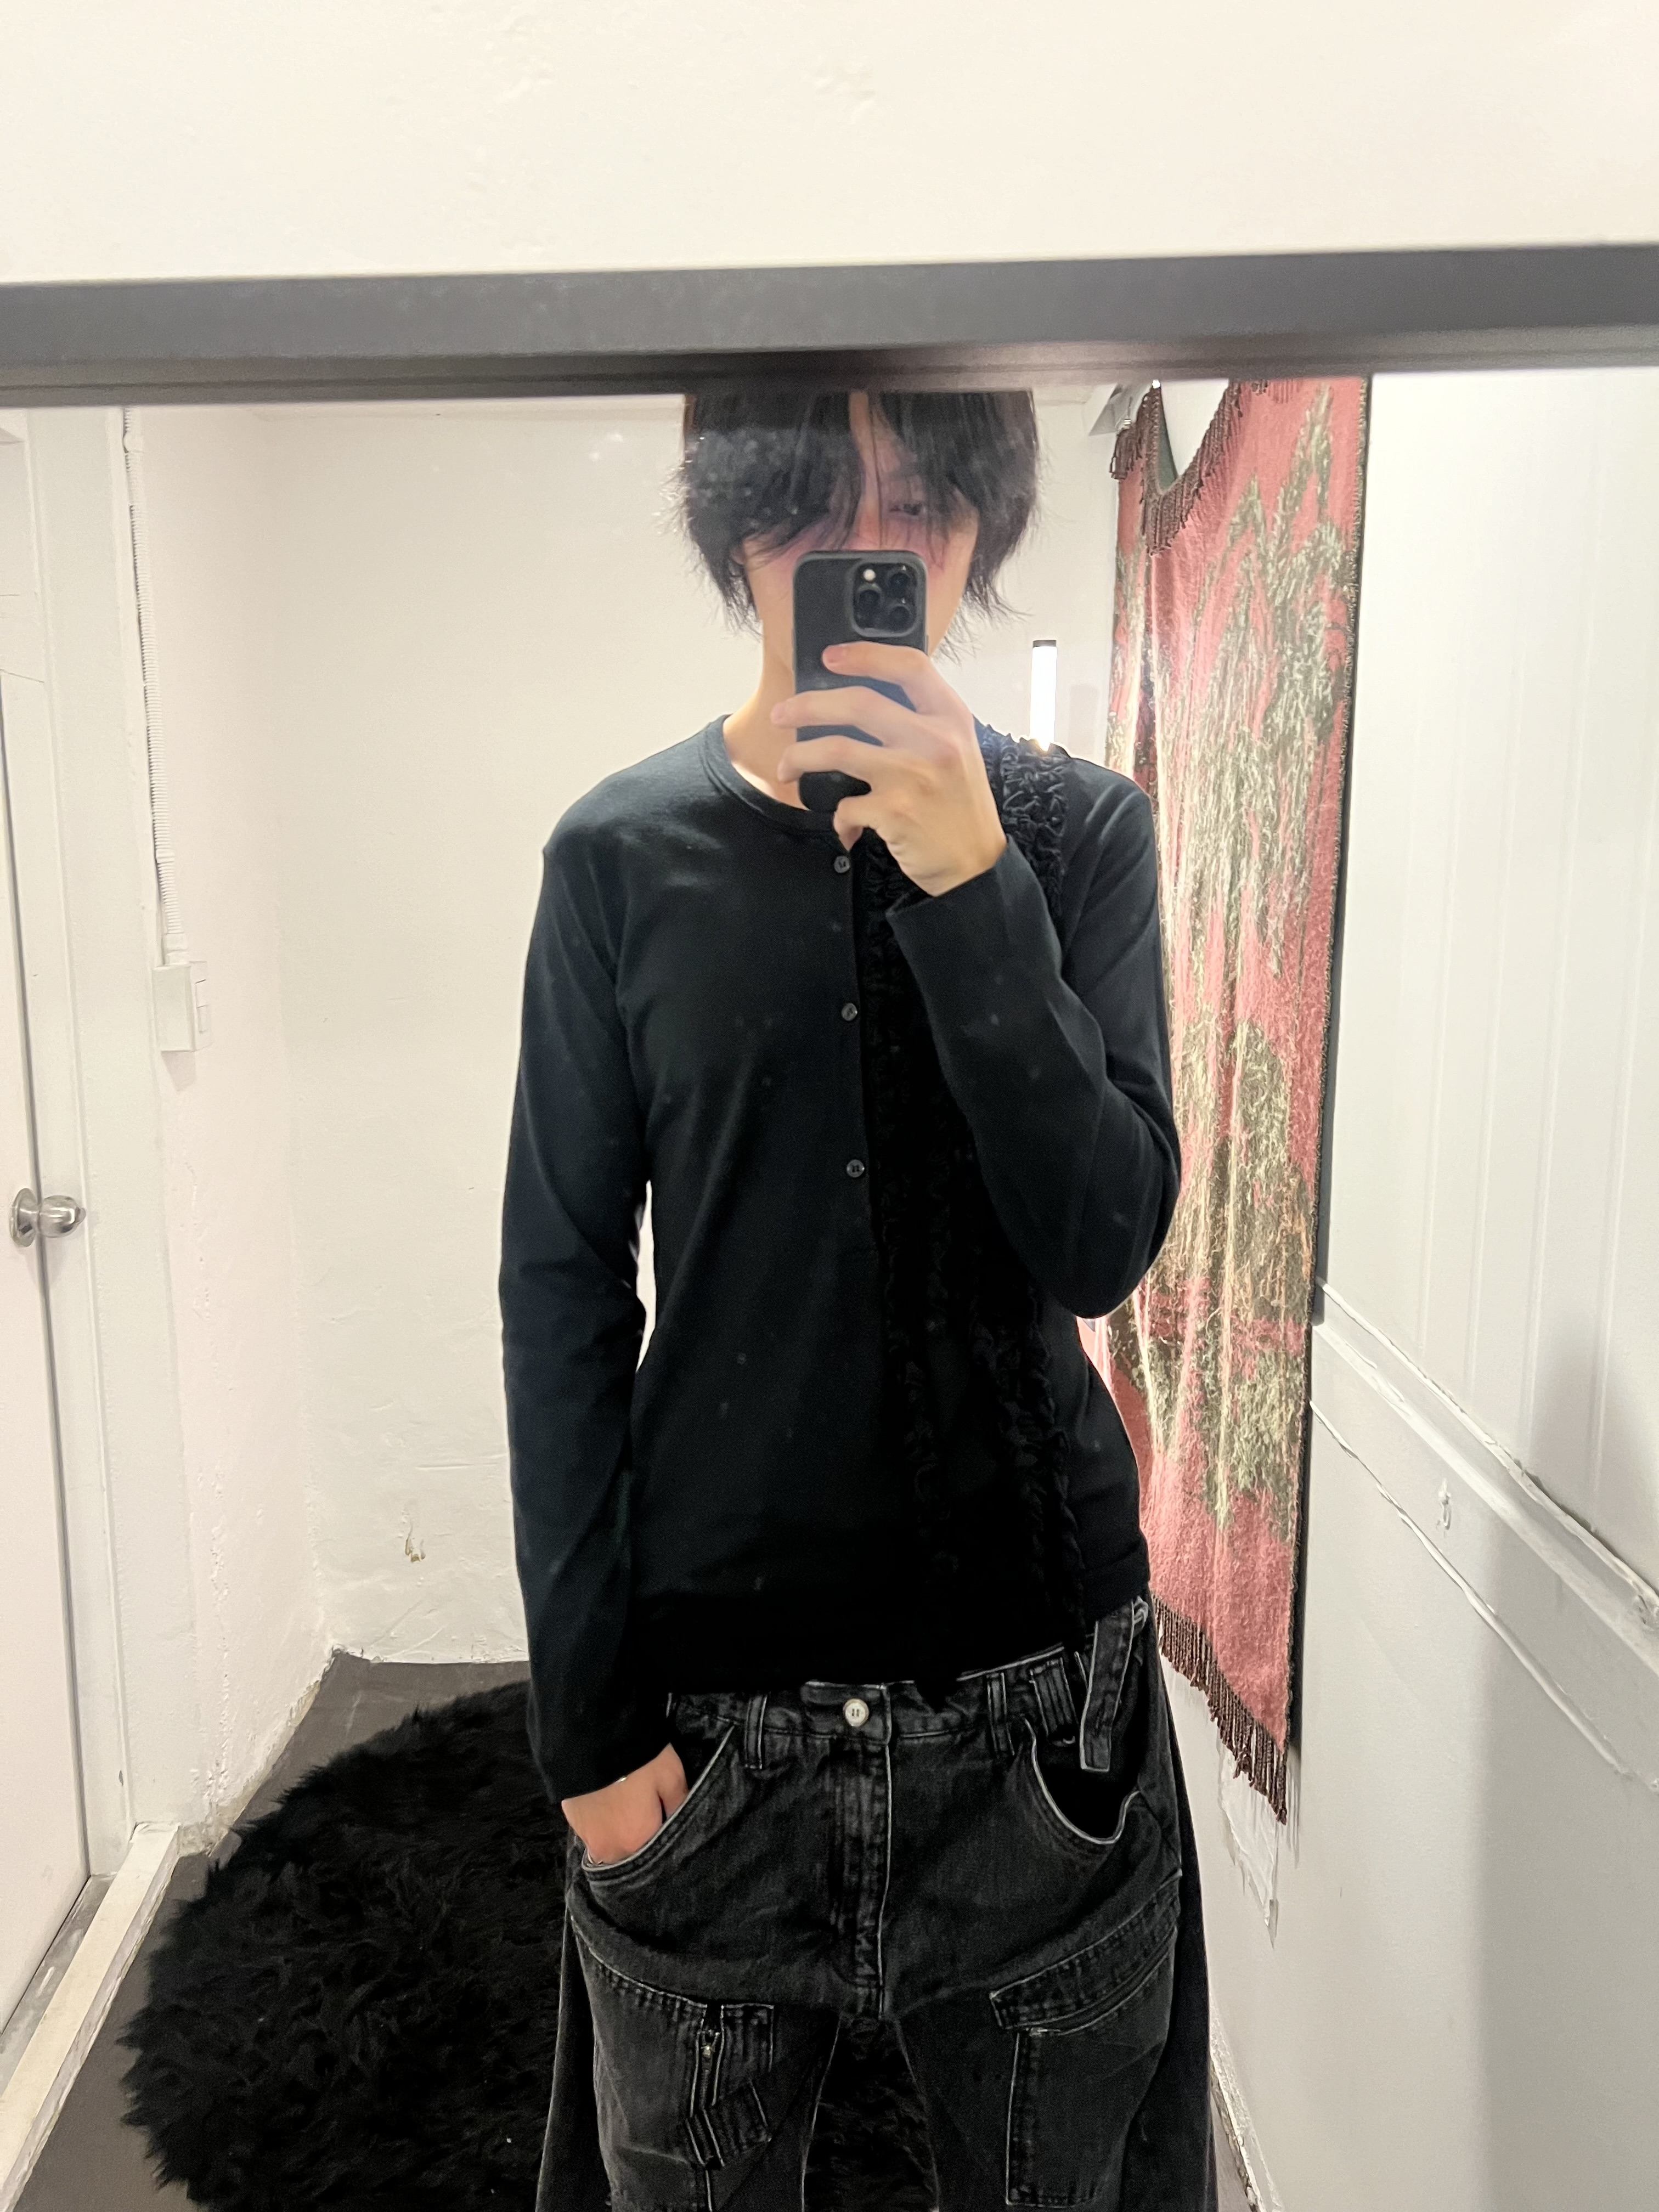
\includegraphics[width=\textwidth]{styled_pics/12.jpg}
        \caption*{Yohji Yamamoto Pour Homme, Y/Project}
    \end{figure}
\end{minipage}
\begin{minipage}[h!]{0.5\textwidth}
    \begin{figure}[H]
        \includegraphics[width=\textwidth]{styled_pics/13.jpg}
        \caption*{Edward Cuming, Craig Green, Comme des Garcons Homme Plus}
    \end{figure}
\end{minipage}
\begin{minipage}[h!]{0.5\textwidth}
    \begin{figure}[H]
        
\includegraphics[width=\textwidth]{styled_pics/14.jpg}
        \caption*{GmbH, Comme des Garcons BLACK, 10 Corso Como}
    \end{figure}
\end{minipage}
\begin{minipage}[h!]{0.5\textwidth}
    \begin{figure}[H]
        \includegraphics[width=\textwidth]{styled_pics/15.jpg}
        \caption*{Comme des Garcons BLACK, GmbH}
    \end{figure}
\end{minipage}
\begin{minipage}[h!]{0.5\textwidth}
    \begin{figure}[H]
        \includegraphics[width=\textwidth]{styled_pics/16.jpg}
        \caption*{1017 ALYX 9SM, TheSoloist.}
    \end{figure}
\end{minipage} 



% End document
\end{document}